%%%%%%%%%%%%%%%%%%%%%%%%%%%%%%%%%%%%%%%%%

%----------------------------------------------------------------------------------------
%       Paquetes y configuraciones
%----------------------------------------------------------------------------------------

\documentclass[11pt, a4paper]{article} % Font size
\usepackage[sfmath]{kpfonts}
\renewcommand*\familydefault{\sfdefault}

\usepackage{charter} % Use the Charter font for the document text
\usepackage[utf8]{inputenc}
\usepackage[T1]{fontenc}
\usepackage[spanish,es-nolayout,es-nodecimaldot,es-tabla]{babel}
\usepackage{amsmath}
\usepackage{subfigure}
\usepackage{amsfonts}
\usepackage{amssymb,amsthm}
\usepackage{enumerate}
\usepackage{enumitem}
\usepackage{parskip}
\usepackage{listings}
\usepackage{nicefrac}
\usepackage{framed, color}
\usepackage{graphicx}
\usepackage[left=2cm,right=2cm,top=2.5cm,bottom=2cm]{geometry}
\usepackage[colorlinks = true]{hyperref} 
\usepackage{wrapfig}
\usepackage[font={footnotesize,it}]{caption}
% Please add the following required packages to your document preamble:
\usepackage[normalem]{ulem}
\useunder{\uline}{\ul}{}
\usepackage{cancel}
%
%       Configuración de Problema y Proposición
%
\definecolor{db}{RGB}{0,128,128}                % Color de pregunta y respuesta
\definecolor{dg}{RGB}{128,0,128}                % Color de proposiciones y teoremas
\definecolor{dh}{RGB}{128,128,0}                % Color de preguntas adicionales
\definecolor{da}{RGB}{0,102,153}                % Color de direcciones electrónicas
\newtheorem{teo}{Teorema}

\newtheoremstyle{dotlessP}{1em}{\topsep}{\color{db}}{}{\color{db}\bfseries}{}{ }{}
\theoremstyle{dotlessP}
\newtheorem*{prob}{Problema:}

\newtheoremstyle{dotlessS}{1em}{\topsep}{\color{dg}}{}{\color{dg}\bfseries}{}{ }{}
\theoremstyle{dotlessS}
\newtheorem*{prop}{Proposición:}


% Comandos
\newcommand{\R}{\mathbb{R}}
\newcommand{\dsum}{\displaystyle \sum}
\newcommand{\yds}{\qquad\text{y}\qquad}
\DeclareMathOperator{\Dom}{Dom}
\DeclareMathOperator{\Ran}{Ran}
\DeclareMathOperator{\inv}{inv}


% Revisa para posible uso: http://principiae.be/pdfs/TUG-X-004-slideshow.pdf
%---------------------------------------------------------------------------------------------
%       Recursos desarrollados en la Comunidad virtual – Tutoría en línea
%---------------------------------------------------------------------------------------------

% Tipo de documento
\newcommand{\tipodedocumeto}{Curso de preparación al examen Ser bachiller}

% Autor
\newcommand{\autor}{Lissett Castillo}

% Editores
\newcommand{\editores}{Andrés Miniguano Trujillo y Juan Carlos Trujillo}

% Correos electrónicos
\newcommand{\email}{\href{mailto:refasabu@hotmail.com}{\color{da}ana.castillo01@epn.edu.ec}}

\newcommand{\emaila}{\href{mailto:andres.miniguano@epn.edu.ec}{\color{da}andres.miniguano@epn.edu.ec}}

\newcommand{\emailb}{ y \href{mailto:jcto36@gmail.com}{\color{da}jcto36@gmail.com}}

% Fecha de creación de la pregunta
\newcommand{\creacion}{5 de abril de 2017}

% Fecha de publicación del recurso
\newcommand{\publicacion}{5 de abril de 2017}

% Título del recurso
\newcommand{\titulo}{Preguntas}


\usepackage{fancyhdr}
\pagestyle{fancy}
\renewcommand{\headrulewidth}{0pt}
\chead{\titulo}


\usepackage{lastpage}
\cfoot{\thepage\ de \pageref{LastPage}}


%----------------------------------------------------------------------------------------

\begin{document}\thispagestyle{empty}

\begin{center}

\includegraphics[width=0.5\linewidth]{logos.pdf}
\end{center}


\begin{flushleft}

\large
\rule{\textwidth}{1pt} \vspace{-1em} \par \noindent
\centerline{\LARGE                                      \tipodedocumeto                 } 
\vspace{-0.75cm} \par\noindent%
\rule{\textwidth}{1pt} \par \noindent
%
%
\setlength{\tabcolsep}{0pt}%
%
\begin{tabular}{l@{\hspace{1em}}l}%
        \textbf{Autor:}                 &        \autor \, (\email) \\
        \textbf{Editores:}               &        \editores                                \\
                                                & Proyecto CLAVEMAT              \\ 
                                                & Escuela Politécnica Nacional  \\
        \textbf{Email:}                  & \emaila                \emailb                                  \\
        \textbf{Creación:}               &  \creacion                             \\
        \textbf{Publicación:}            &  \publicacion
\end{tabular}%
\end{flushleft}
%
%
\rule{\textwidth}{1pt}  \vspace{-1em} \par \noindent
\centerline{\textbf{\Large              \titulo                 }} \vspace{-1em}
\rule{\textwidth}{1pt}  \vspace{1em} \par

%----------------------------------------------------------------------------------------
%       Contenidos
%----------------------------------------------------------------------------------------

\begin{enumerate}[label=\color{dg}\theenumi.]
 \setcounter{enumi}{5}
  \normalsize
  %------------- PREGUNTA 6 ---------------------------------------------------------------------------
   \item {\color{db}En la tabla se observan las 			prendas que tiene Nancy en su armario. Si se 			escoge 	una prenda al azar, ¿cuál es la 				probabilidad de que 	sea una blusa color rojo?
        }
        
	\begin{table}[htbp]
		\centering
		\label{my-label}
	\begin{tabular}{|c|c|c|}
		\hline
		\textbf{Número} & \textbf{Prenda} & 					\textbf{Color} \\ \hline
		5               & Blusas          & Rojo         		  \\ \hline
		2               & Blusas          & Azul          		 \\ \hline
		4               & Pantalones      & Negro          \\ 		\hline
		3               & Pantalones      & Plomo          \\ 		\hline
		1               & Falda           & Rosado         \\ 		\hline
		6               & Chaquetas       & Negro          \\ 		\hline
	\end{tabular}
	\end{table}
    \(
     {\color{dh} \textbf{1)} \quad \dfrac{1}{21}} \vspace{1\baselineskip} \\ 	
     {\color{dh} \textbf{2)} \quad \dfrac{2}{21}} \vspace{1\baselineskip} \\ 	
     {\color{dh} \textbf{3)} \quad \dfrac{5}{21}} \vspace{1\baselineskip} \\ 	
     {\color{dh} \textbf{4)} \quad \dfrac{6}{21}}   \vspace{1\baselineskip} \\ 	
      \)
      \textbf{Solución} \\
    Determina \textbf{B} al evento \textbf{<<blusas dhe 			color rojo>>} en la tabla existen \(5\) blusas de color 	rojo que conforman el evento B. Ahora denomina \textbf{T} 		al evento \textbf{<<total prendas existentes en el 		armario de Nancy>>}, sumando los resultado de la tabla 		existen: \(5 + 2 + 4 + 3 + 1 + 6 = 21\) prendas que 		conforman T.
	\\
	La probabilidad de B viene dado por la regla de Laplace: 	número de casos favorables sobre casos posibles, es decir 		\textbf {\(p\,(B) = \dfrac{5}{21}.\)}\\
	{\color{dh} La respuesta correcta es la 3.}
%------------- PREGUNTA 7 ---------------------------------------------------------------------------
	\item {\color{db} Tres obreros cavan en 24 horas una 		zanja de 12 m. ¿Cuántos metros cavarán en 12 horas 9 		obreros?
        }
        \(
\vspace{1\baselineskip} \\ 	
     {\color{dh} \textbf{1)} \quad 2} \vspace{1\baselineskip} \\ 	
     {\color{dh} \textbf{2)} \quad 6} \vspace{1\baselineskip} \\ 	
     {\color{dh} \textbf{3)} \quad 18} \vspace{1\baselineskip} \\ 	
     {\color{dh} \textbf{4)} \quad 72}   \vspace{1\baselineskip} \\ 	
      \)
        \textbf{Solución} 
	\\ Dado que trés obreros  trabajando juntos por 24 horas 	cavan una zanja de 12 metros, es decir, un obrero cavara 4 		metros.  Debes realizar una regla de trés simple para 		reducer el tiempo de trabajo a  12 horas.       
	\begin{table}[htbp]
	\centering
		\begin{tabular}{cccc}
		\textbf{24 horas} & \textbf{4 metros} &             &                  \\
		\textbf{12 horas} & \textbf{x}        & = 					$\displaystyle\frac{12 \cancel{\,horas} \times 4 			metros }{24 \cancel {\,horas}}$ & \textbf{= 2 metros}
		\end{tabular}
	\end{table}
 	\\ 
	Entonces un hombre trabajando 12 horas  cavará 2 metros, 	al contar con 9 obreros, realizas la siguiente regla de 	trés simple.
	\begin{table}[htbp]
	\centering
		\begin{tabular}{cccc}
		\textbf{1 obrero} & \textbf{2 metros} &             &                  \\
		\textbf{9 obreros} & \textbf{x}      &= 					$\displaystyle\frac{9 \cancel{\,obreros} \times 2 			metros }{1 \cancel {\,obrero}}$ & \textbf{= 18 				metros}
 		\end{tabular}
	\end{table}
       \\
	Los 9 obreros trabajando juntos cavarán 18 metros en 12 	horas.    \\
	{\color{dh} La respuesta correcta es la 3.}
	\\
%------------- PREGUNTA 8 ---------------------------------------------------------------------------
\item {\color{db} En un laboratorio se lleva un registro del número de bacterias, en millones, que crecen en función del tiempo para dos muestras diferentes. Si la primera muestra se encuentra expresada por \(2^{4t}\) y  la segunda mediante \(4^t (16^{1 - 3t})\), donde \(t\) representa el tiempo en minutos. Determine el tiempo en el que las muestras son iguales.}
   \(
\vspace{1\baselineskip} \\ 	
     {\color{dh} \textbf{1)} \quad \dfrac{1}{6}} \vspace{1\baselineskip} \\ 	
     {\color{dh} \textbf{2)} \quad \dfrac{2}{9}} \vspace{1\baselineskip} \\ 	
     {\color{dh} \textbf{3)} \quad \dfrac{2}{7}} \vspace{1\baselineskip} \\ 	
     {\color{dh} \textbf{4)} \quad \dfrac{5}{2}}   \vspace{1\baselineskip} \\ 	
      \)
      \textbf{Solución} 
    \\ Debes igualar las muestras como estan a continuacion, para determinar el tiempo donde las muestras son las mismas:
\[
2^{\,4t}  = 4^t(\,16^{\,(1 - 3t)})
\]
El objetivo es despejar \(t\), entonces: 
\begin{align*}
2^{\,4t}  &= 2^{\,2t}(2^{\,4(1 - 3t)})   &{\text{El coeficiente 4 lo expresas, en base 2 con exponente 2.}}  
\\
\dfrac{2^{\,4t}}{2^{\,2t}}  &=  2^{\,4(1 - 3t)}  &{\text{El término}\, {2^{\,2t}}  \text{ pasa a dividir a la primera muestra.}} 
\\
2^{\,4t-2t}  &= 2^{\,4 - 12t} &\text{Aplicas las propiedades de división de fracciones.}  
\\
2^{\,2t}  &= 2^{\,4 - 12t} &{\text{ Siendo} \,\, {2^{\,2t}}  \text{ el resultado de la diferencia de fracciones.}} 
\\
\log 2^{\,2t}  &= \log 2^{\,4 - 12t} &\text{Aplicas las propiedades de logaritmo.}  
\\
2t  &= 4 - 12t &\text{Esto hace que las bases se simplifiquen por ser iguales}  
\\
2t +  12t&= 4 &\text{Así también los exponentes bajan.}  
\\
14t&= 4  &\text{Despejas t.}  
\\
t &= \displaystyle\frac{\cancel 4}{\cancel 14} &\text{Simplicas la fracción.}  
\\
t &= \dfrac{2}{7} &\text{Y obtienes el resultado.}  
\end{align*}
El tiempo donde las muestras son iguales es $\dfrac{2}{7}$ minutos.
\\
{\color{dh} La respuesta correcta es la 3.}
\\
%------------- PREGUNTA 9 ---------------------------------------------------------------------------
\item {\color{db} El aumento en el número de artículos que se venden en una tienda en los primeros días del mes de diciembre se representan mediante la expresión: 
\[
3^x = 243
\]
Si x representa los días, determine el día en el que el incremento en ventas es igual a 243 artículos.}
        \(
\vspace{1\baselineskip} \\ 	
     {\color{dh} \textbf{1)} \quad 2} \vspace{1\baselineskip} \\ 	
     {\color{dh} \textbf{2)} \quad 3} \vspace{1\baselineskip} \\ 	
     {\color{dh} \textbf{3)} \quad 4} \vspace{1\baselineskip} \\ 	
     {\color{dh} \textbf{4)} \quad 5}   \vspace{1\baselineskip} \\ 	
      \)
        \textbf{Solución} \\
En la ecuación tenemos el 3 elevado a la potencia \( x \), para encontrar el valor de \( x \) debes probar cuantas veces el numero 3 debería ser multiplicado por sí mismo para que sea igual a \( 243\).
Entonces probamos:
\begin{align*}
\textbf{Si} \quad & x = 3 &\quad 3^3 = &\quad 3\, x\, 3\, x\, 3\, =\, 27 \\
            & x = 4 & 3^4 = &\quad 3\, x\, 3\, x\, 3\, x\, 3\, =\, 81\\
            & x = 5 & 3^5 = &\quad 3\, x\, 3\, x\, 3\, x\, 3\, x\, 3\, =\, 243 
\end{align*}

El valor de \( x \) es 5, siendo el quinto día donde el incremento en ventas es igual a 243 artículos.\\
{\color{dh} La respuesta correcta es la 4.}
\\
%------------- PREGUNTA 10 ---------------------------------------------------------------------------
\item {\color{db} Con base en el gráfico que muestra la posición de dos barcos, respecto a los observadores en \((1; 1)\) para $\vec{a}$ y \((-2; -1)\) para $\vec{b}$.
 \begin{center}
	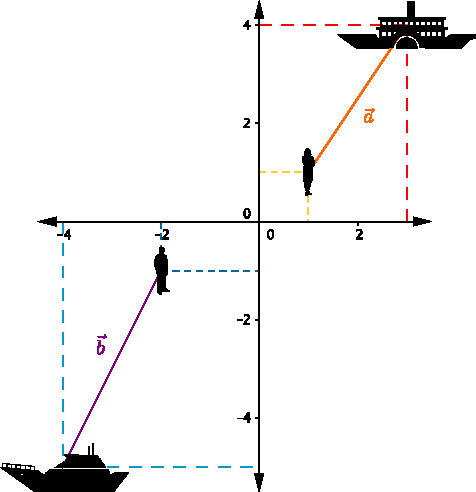
\includegraphics[scale=0.7]{Figuras/10.pdf}
\end{center}
Determine el vector $2$$\vec{a} + \vec{b}$ correspondiente al desplazamiento que realizará el barco $\vec{a}$ cuando duplique su desplazamiento con respecto al barco $\vec{b}$.
        }
 \(
\vspace{1\baselineskip} \\ 	
     {\color{dh} \textbf{1)} \quad (2i,3j)} \vspace{1\baselineskip} \\ 	
     {\color{dh} \textbf{2)} \quad (-2i,-4j)} \vspace{1\baselineskip} \\ 	
     {\color{dh} \textbf{3)} \quad (2i,2j)} \vspace{1\baselineskip} \\ 	
     {\color{dh} \textbf{4)} \quad (-2i,-3j)}   \vspace{1\baselineskip} \\ 	
      \)
        \textbf{Solución} 
\\ Mediante el gráfico el obeservador A se encuentra en el punto \((1; 1)\) y el barco A en el punto \((3; 4)\), mientras que el obeservador B se encuentra en el punto \((-2 ; -1)\) y el barco B en el punto \((-4; -5)\).
\\ Debes calcular el vector $\vec{a}$ realizando la diferencias entre la posición del barco y la posición del observador; y para que sea un vector debes multiplicarlo por un vector unitario de magnitud 1: 
\begin{align*}
\vec{a} &=[(3, 4)-(1, 1)]*(i,j)
\\
\vec{a} &=[(3-1),(4-1)]*(i,j)
\\
\vec{a} &=[(2),(3)]*(i,j)
\\
\vec{a} &=(2i,3j)
\end{align*}
\\ Para el vector $\vec{b}$ es el mismo procedimiento. 
\begin{align*}
\vec{b} &=[(-4, -5)-(-2, -1)]*(i,j)
\\
\vec{b} &=[(-4-(-2)),(-5-(-1)]*(i,j)
\\
\vec{b} &=[(-4+2),(-5+1)]*(i,j)
\\
\vec{b} &=[(-2),(-4)]*(i,j)
\\
\end{align*}
Ahora que cuentas ya con los vectores \(\vec {a}\) y \(\vec {b}\) puedes determinar el desplazamiento \(2 \vec{a} + \vec {b}\), el cual debes multiplicar al vector \(\vec {a}\) por 2 y sumarle al vector \(\vec {b}\).
\begin{align*}
2 \vec{a} + \vec{b} &=2*(2i,3j) + (-2i,-4j)
\\
&=(2*2i,2*3j) + (-2i,-4j)
\\
&=(4i,6j) + (-2i,-4j)
\\
&=(4i-2i) + (6j-4j)
\\
&=(2i + 2j)
\end{align*}
\\
{\color{dh} La respuesta correcta es la 3.}
\\
\end{enumerate}

%----------------------------------------------------------------------------------------
\begin{enumerate}[label=\color{dg}\theenumi.]
 \setcounter{enumi}{128}
  \normalsize
  %------------- PREGUNTA 129 -----------------------------------------------------------------
   \item {\color{db} Con base en la vista lateral de la figura, identifique a qué sólido corresponde.  } \\
	     \begin{center}
    
\includegraphics[scale=1]{Figuras/129_1.pdf}
    \end{center}
        \begin{figure}[h!]
       \centering
       \subfigure[]{\label{fig:a}
\includegraphics[scale=1]{Figuras/129_2-1.pdf}}\qquad 
		\subfigure[]{\label{fig:b}
\includegraphics[scale=1]{Figuras/129_2-2.pdf}}\qquad 
        		\subfigure[]{\label{fig:c}
\includegraphics[scale=1]{Figuras/129_2-3.pdf}}\qquad 
                		\subfigure[]{\label{fig:d}
\includegraphics[scale=1]{Figuras/129_2-4.pdf}}
\end{figure}
 \textbf{Solución}\\
 Observas la parte lateral de cada una de las figuras sus vistas laterales, la opción \textbf{a}  es un rectangulo y su vista lateral solo contiene dos divisiones, en la opción \textbf{b}  es un cilindro el cual su vista lateral es una sola división, la opción \textbf{c}  esta es un poliedro regurar y su vista lateral contiene 3 divisiones siendo igual a la inicial.
 \\
 {\color{dh} La respuesta correcta es la c.}
 
          %------------- PREGUNTA 130 -----------------------------------------------------------------
   \item {\color{db} Identifique el gráfico que corresponde a la vista lateral derecha de la figura bidimensional. \\
        }
             \begin{center}
    
\includegraphics[scale=1]{Figuras/130_1.pdf}
    \end{center}
    
         \begin{figure}[h!]
       \centering
       \subfigure[]{\label{fig:a}
\includegraphics[scale=1]{Figuras/130_2-1.pdf}}\qquad 
		\subfigure[]{\label{fig:b}
\includegraphics[scale=1]{Figuras/130_2-2.pdf}}\qquad 
        		\subfigure[]{\label{fig:c}
\includegraphics[scale=1]{Figuras/130_2-3.pdf}}\qquad 
                		\subfigure[]{\label{fig:d}
\includegraphics[scale=1]{Figuras/130_2-4.pdf}}
\end{figure}
 \textbf{Solución}\\
 Te debes fijar en cada uno de los detalles de la figura bidimensional, uno de ellos que es muy notorio son sus bordes superiores los cuales estan redondeados y la unica opción que cumple con ello es la e\\
 {\color{dh} La respuesta correcta es la e.}
  %------------- PREGUNTA 131 -----------------------------------------------------------------
   \item {\color{db} Identifique la imagen que se obtiene al girar la figura 90º en sentido horario.
        }
         \begin{center}
    
\includegraphics[scale=1]{Figuras/131_1.pdf}\\
    \end{center}
    
      \begin{figure}[h!]
       \centering
       \subfigure[]{\label{fig:a}
\includegraphics[scale=1]{Figuras/131_2-1.pdf}}\qquad 
		\subfigure[]{\label{fig:b}
\includegraphics[scale=1]{Figuras/131_2-2.pdf}}\qquad 
        		\subfigure[]{\label{fig:c}
\includegraphics[scale=1]{Figuras/131_2-3.pdf}}\qquad 
                		\subfigure[]{\label{fig:d}
\includegraphics[scale=1]{Figuras/131_2-4.pdf}}
\end{figure}
 \textbf{Solución} \ \
 El giro que te piden es en sentido horario con lo que debes girar una sola vez hacia la derecha. \\
 {\color{dh} La respuesta correcta es la i}
  %------------- PREGUNTA 132 -----------------------------------------------------------------
   \item {\color{db} Identifique la imagen que continúa  la secuencia. 
        }
         \begin{center}
    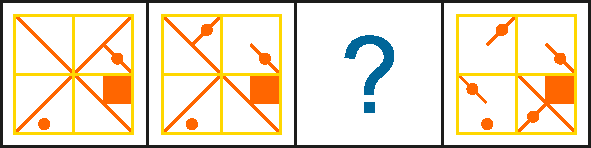
\includegraphics[scale=1]{Figuras/132_1.pdf}
    \end{center}
    
    \begin{figure}[h!]
       \centering
       \subfigure[]{\label{fig:a}
\includegraphics[scale=1]{Figuras/132_2-1.pdf}}\qquad 
		\subfigure[]{\label{fig:b}
\includegraphics[scale=1]{Figuras/132_2-2.pdf}}\qquad 
        		\subfigure[]{\label{fig:c}
\includegraphics[scale=1]{Figuras/132_2-3.pdf}}\qquad 
                		\subfigure[]{\label{fig:d}
\includegraphics[scale=1]{Figuras/132_2-4.pdf}}
\end{figure}
 \textbf{Solución} \\
Debes observar cada uno de los elementos de la secuencia, tenemos que la secuencia empieza con una linea divisora por cuadrante que va en sentido  antihorario, el numero de puntos  va aumentando en igual sentido horario y el cuadro permanece constante.  Entonces el cuadrante faltante  debes tener en cuenta que para el paso 3 de la secuencia contiene solo dos lineas  en sus cuadrantes inferiores y el unico que cumple esa condición es la opción p.\\ 
{\color{dh} La respuesta correcta es la p.}
\end{enumerate}

%Ser_Bachiller_129_Fig_p
\end{document}